\section{Known Issues}
\label{chap:issues}
\paragraph{An API baseline has not been set for this Workspace}
\begin{enumerate}
\item Go to the Eclipse Problems View ($Window\rightarrow Show View\rightarrow Problems$)
\item Right click the 'API baseline' error 
\item In the context menu select $Quick Fix$
\item A Preference Window filtered for the API Baselines opens up
\item in that Dialog find the field $Missing API Baseline$ and set it to $Ignore$
\begin{figure}[H]
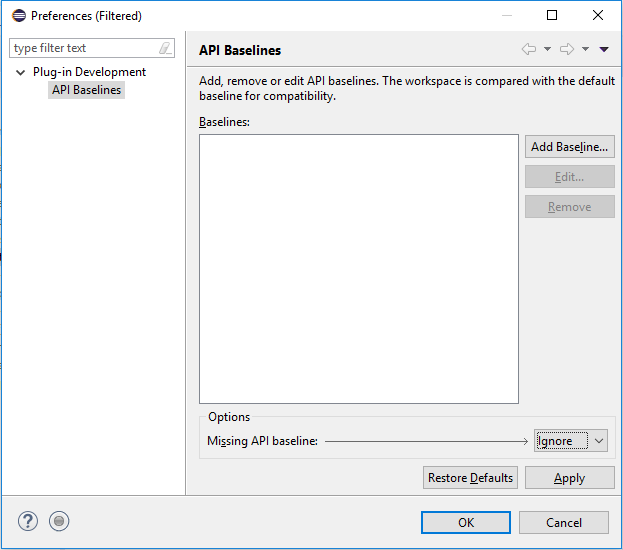
\includegraphics[scale=0.5]{images/ignoreAPIError.png}

\end{figure}
\end{enumerate}
\paragraph{Plugin Execution not covered by lifecycle configuration} 
\begin{enumerate}
\item Go to $Window\rightarrow Preferences\rightarrow Maven\rightarrow Error/Warnings$
\item find the line 'Plugin Execution not covered..'
\item Set the Value to ignore, by choosing selecting 'ignore' in the combo box
\item Click on Apply/Ok to rebuild the projects
\end{enumerate} 
\paragraph{When cloning into/ importing xstampp and its sub projects to eclipse the project dependencies must be located sometimes}
\begin{enumerate} 
\item In the Project Explorer right click on the project 'Build Path->Configure Build Path'
\item In the 'Java Build Path' Page click on 'Source', by doing that java relocates the source folders in the projects andsets the dependencies
\item hit Apply/Ok to store the settings
\end{enumerate} 